The aim of this chapter is to introduce \textit{control methods} for \textbf{spacecraft}, then we will include the spacecraft (described by Dynamic-Kinematic equations) in a \textbf{feedback loop}. The \textit{Attitude Control System} is in charge to:
\begin{enumerate}
    \item Give a proper orientation to the body
    \item Stabilize the spacecraft about a reference in the presence of disturbance torques.
\end{enumerate}
\begin{quote}
    \textsf{
        Important: The Attitude orientation is fundamental in any space mission.
    }
\end{quote}

\begin{figure}[h]
    \centering
    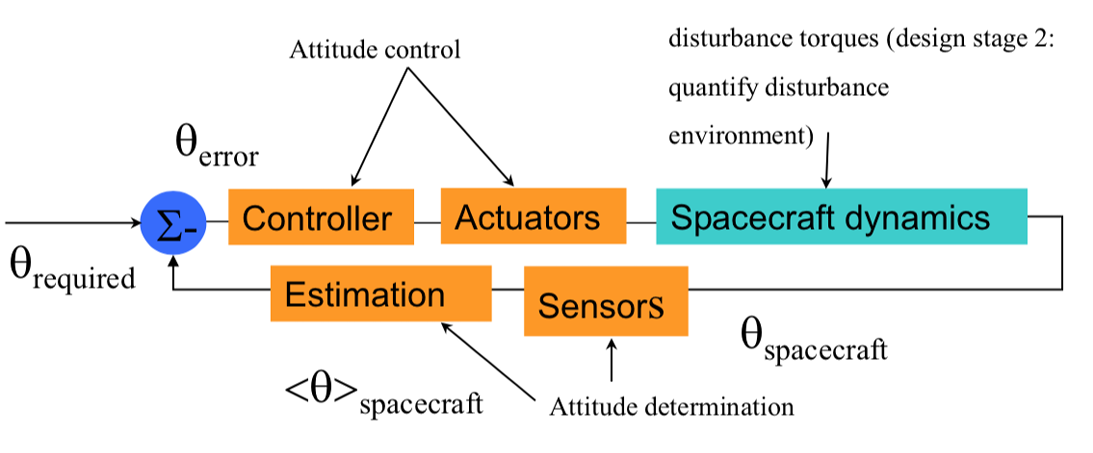
\includegraphics[scale=0.6]{AerospaceApplications/images/ACS.png}
    \caption{Attitude Control System}
\end{figure}

\section{Sensors}
A \textbf{sensor} employed in this field must be able to provide \textbf{in real time} the measurement of the attitude. This is fundamental to build any effective control system. The available sensors can be broken into two families:
\begin{itemize}
    \item \textbf{Absolute attitude sensors} which determine the attitude with respect to some celestial body like the Sun or other stars (an example can be a \textbf{star tracker}).
    \item  \textbf{Relative attitude sensors} they are capable to measure the \textit{angular rate}, then the attitude is obtained through integration (they are usually \textbf{gyroscopes}).
\end{itemize}

\section{Actuators}
An \textbf{actuator} is fundamental in order to give to the system to control (the spacecraft) the \textbf{control input}. Even here three groups of actuators can be distinguished:
\begin{enumerate}
    \item \textbf{Dampers} which are used to reduce the effect of nutation and external disturbances torques;
    \item \textbf{Actuators which provides external torques}, they include \textit{thrusters, reaction wheels, particular types of Gyros};
    \item \textbf{Actuators which use external forces} like magnetic fields, gravity gradient and so on.
\end{enumerate}
The control laws we will present can be applied by using thrusters, reaction wheels or combination of them.

\section{Control system approaches}
How it has been mentioned in the introduction, the main objective of an attitude control system can be the \textbf{stabilization} about a reference attitude, or the tracking in the case that the orientation changes in time.
We can split the \textit{attitude control systems} in three categories:
\begin{enumerate}
    \item \textsc{Passive}: they are based on enviromental forces and on the properties of the body. They exist because environment perturbations can lead to stable behaviours. Passive control systems are seldom used.
    \item \textsc{Semi-active}, in this case some \textit{reaction wheels} are used that exploit the angular momentum consevation. Alternatively can be used \textit{magnetic systems} which interacting with the magnetic field tend to produce useful torques.
    \item \textsc{Active}: is the most used in the field of ACS (Attitude Control Systems), the technique is based on the use of \textit{thrusters}.
\end{enumerate}
\begin{quote}
    \textsf{
        A lot of classifications are available, another possible classification is that beetween: \textit{Spin stabilization} and \textit{3-axis stabilization}. The presented approach is based on \textbf{Three-axis control}.
    }
\end{quote}

\section{Attitude control: a general setting}
In the previous chapter we have seen the equations for dynamics and kinematics of a spacecraft, moreover we have understood that a useful and effective description of the orientation can be provided by  \textit{quaternions}, as they are powerful and \textit{gimbal lock free}.\\
The \textbf{general goal} of \textit{control} is to make the state vector $(\mathfrak{q}, \boldsymbol{\omega})$ track a \textbf{reference vector} $(\mathfrak{q}_r, \boldsymbol{\omega_r})$ which can be eventually time-varying. In order to determine what is the 'distance' from the desired behaviour we have to compute the tracking error:
\begin{itemize}
    \item The \textbf{angular velocity tracking error} is defined simply as
    \begin{equation*}
        \tilde{\boldsymbol{\omega}} \doteq \boldsymbol{\omega}_r - \boldsymbol{\omega}
    \end{equation*}
    \item The \textbf{quaternion tracking error} is defined as a product beetween quaternions
    \begin{equation*}
        \tilde{\mathfrak{q}} \equiv \begin{bmatrix}
          \   \tilde{q_0} \ \\\ \tilde{\mathbf{q}} \
        \end{bmatrix} \doteq \mathfrak{q}^{-1} \otimes \mathfrak{q}_r = \mathfrak{q}^* \otimes \mathfrak{q}_r
    \end{equation*}
    The quaternion $\tilde{\mathfrak{q}}$ is nothing but the quaternion which starting from $\mathfrak{q}$ goes to $\mathfrak{q}_r$. 
\end{itemize}

\section{First problem: Regulation (PD control law)}
The \textit{goal of regulation} is obtaining
\begin{align*}
    &\mathfrak{q} \to \mathfrak{q}_r = const  \quad \text{and} \quad \boldsymbol{\omega}\to0\\
    &\tilde{\mathfrak{q}}\to\mathfrak{I}\doteq(1,\mathbf{0}) \quad \text{and} \quad \boldsymbol{\tilde{\omega}}\to0
\end{align*}
This is the simplest problem of control with respect to the other, because the quaternions to reach is constant and then does not change in time.\\
A  \textbf{simple linear control  law} is
{\large{
    \begin{equation}
        \mathbf{u} = k_p\tilde{\mathbf{q}}-k_d\boldsymbol{\omega}
    \end{equation}
}}
where $k_p>0$ and $k_d>0$ are parameters to tune. Note that in this law enters only the vector part of the \textit{quaternion tracking error}, and the law it is substantially a Proporzional-Derivative (PD) one, where you have a term \textbf{proportional} to $\tilde{\mathbf{q}}$ and a term which depends by a constant $k_d$ by the derivative.\\
In general the Kinematic-Dynamic equations are:
{\large{
    \begin{align*}
        &\dot{\mathfrak{q}} = \frac{1}{2}\mathbf{Q}\boldsymbol{\omega}\\
        &\dot{\boldsymbol{\omega}} = -\mathbf{J}^{-1}\boldsymbol{\omega} \times \mathbf{J}\boldsymbol{\omega}+\mathbf{J}^{-1}\mathbf{u}
    \end{align*}
}}
By applying the control law we have just introduced, we will obtain:
{\large{
    \begin{align*}
        &\dot{\tilde{\mathfrak{q}}} = -\frac{1}{2}\boldsymbol{\omega}^q \otimes \tilde{\mathfrak{q}}\\
        &\dot{\boldsymbol{\omega}} = -\mathbf{J}^{-1}(-\boldsymbol{\omega} \times \mathbf{J}\boldsymbol{\omega}+k_p\tilde{\mathbf{q}}-k_d\boldsymbol{\omega})
    \end{align*}
}}

The defined system has \textbf{two equilibria} associated with the same attitude, specifically they are $(\tilde{q_0}, \tilde{\mathbf{q}}, \boldsymbol{\omega})=(\pm1,\mathbf{0, 0})$, this is why it is the same cosine function whose arguments are different each for an angle equal to $\pi$, by using the trigonometry it is easy to show it.\\
Reguarding such equilibria, an important theorem holds:\\

\hspace*{-5mm}
\begin{tikzpicture}
\node [mybox] (box){%
    \begin{minipage}{.96\textwidth}     %Larghezza del box
    {\large{
        \textbf{Theorem}\\
        The equilibrium points $(\pm1, \mathbf{0, 0})$ of the \textit{closed-loop system} are \textbf{locally asympotically stable}, moreover for any initial condition $(q_0(0), \tilde{\mathbf{q}}(0), \boldsymbol{\omega}(0))$, \\
        \begin{equation*}
            \lim_{t\to\infty} (q_0(t), \tilde{\mathbf{q}}(t), \boldsymbol{\omega}(t)) = (\pm1, \mathbf{0, 0})
        \end{equation*}
    }}
    \end{minipage}
};
\end{tikzpicture}%

\vspace{0.5cm}
\noindent
The proof is based on the \textit{Lyapunov function}
\begin{equation*}
    V = \frac{1}{4}\boldsymbol{\omega}^T J \boldsymbol{\omega}+
    \frac{1}{2}k_p \tilde{\mathbf{q}^T}\tilde{\mathbf{q}}+
    \frac{1}{2}k_p(1\mp\tilde{q_0})^2
\end{equation*}

For the problem of regulation, there are other effective control laws which provides a \textbf{shortest path to tracking} (when $\text{sign}(\tilde{q_0})$ appears), or \textbf{better performances} in terms of command activity and time response (when the non linear term $(1\pm \tilde{\mathbf{q}}^T \tilde{\mathbf{q}})$ appears). They are:
\begin{align}
    &\mathbf{u} = k_p\text{sign}(\tilde{q_0})\tilde{\mathbf{q}}-k_d\boldsymbol{\omega}\\
    &\mathbf{u} = k_p\tilde{\mathbf{q}}-k_d(1\pm \tilde{\mathbf{q}}^T \tilde{\mathbf{q}})\boldsymbol{\omega}\\
    &\mathbf{u} = k_p\text{sign}(\tilde{q_0})\tilde{\mathbf{q}}-k_d(1\pm \tilde{\mathbf{q}}^T \tilde{\mathbf{q}})\boldsymbol{\omega}
\end{align}

\section{Second problem: Tracking (Sliding mode control)}
The \textit{goal of tracking} problems is:
\begin{align*}
    &\mathfrak{q}(t)\to\mathfrak{q}_r(t) \quad \text{and} \quad
    \boldsymbol{\omega}\to\boldsymbol{\omega}_r(t)\\
    &\tilde{\mathfrak{q}}\to\mathfrak{I}\doteq(1,\mathbf{0}) \quad \text{and} \quad \tilde{\boldsymbol{\omega}}(t)\to0
\end{align*}
The laws which has been just presented can be used, but you will have poor performances and robustness. On the other hand, an \textbf{effective way} to face the tracking problem is using the \textbf{sliding mode control} that provides, differently than the simpler linear control law, \textbf{high performances} and \textbf{robustness}.
The system to control is:
{\large{
    \begin{align*}
        &\dot{\mathfrak{q}} = \frac{1}{2}\mathbf{Q}\boldsymbol{\omega}\\
        &\dot{\boldsymbol{\omega}} = -\mathbf{J}^{-1}\boldsymbol{\omega} \times \mathbf{J}\boldsymbol{\omega}+\mathbf{J}^{-1}\mathbf{u}
    \end{align*}
}}
\noindent
which is in a sort of \textit{generalized normal form}, and how happens in the great majority of mechanical systems the \textbf{relative degree} is $\gamma=2$.
Remind that when you want to exploit the \textbf{sliding mode control} the steps to follow are:
\begin{enumerate}
    \item The definition of a \textit{sliding surface}; 
    \item The definition of a \textit{feedback law}.
\end{enumerate}

\subsection{Sliding mode control for attitude tracking}
In the expression of the sliding surface, usually appears the tracking error and its derivative in a way that is consistent with the \textit{relative degree} of the system. In our case we have to use the \textbf{(quaternion) tracking error} (more specifically for the purposes we use its vector part), and its derivative that is the \textbf{angular velocity}. The resulting sliding surface is 
{\large{
    \begin{equation}
        \mathbf{s}(\mathbf{q}, \boldsymbol{\omega}, t) = k_2\tilde{\mathbf{q}}+\tilde{\boldsymbol{\omega}}
    \end{equation}
}}
It is known that on such sliding surface the tracking error is null. At this point, having defined the first ingredient for SM control, we have to define a \textbf{control law} $\mathbf{u}_s$ such that the surface is:
\begin{itemize}
    \item \textsc{Invariant}, if the state is on the surface, it must remain on it; 
    \item \textsc{Attractive}, if the stato is \textbf{not} on the surface it will be led on it, in finite time.
\end{itemize}

\subsubsection{Invariance of the surface}
Practically speaking, we have to impose that the derivative of the expression defining the sliding surface is 0, that is $\dot{\mathbf{s}}=0$. The derivative is:
\begin{align*}
    \dot{\mathbf{s}}&=\dot{\boldsymbol{\omega}}_r-\dot{\boldsymbol{\omega}}+k_2\dot{\tilde{\mathbf{q}}}=\\
    &\dot{\boldsymbol{\omega}}_r + \mathbf{J}^{-1}\boldsymbol{\omega} \times \mathbf{J}\boldsymbol{\omega} -
    \boldsymbol{J}^{-1}\mathbf{u} +
    \frac{k_2}{2} (\tilde{q_0}\tilde{\boldsymbol{\omega}}+\tilde{\mathbf{q}}\times (\boldsymbol{\omega}_r+\boldsymbol{\omega}) )
\end{align*}
If we invert this expression with respect to $\mathbf{u}$ we can find (a part of) the control law $\mathbf{u}_s$ that is:
\begin{equation}
    \mathbf{u}_s = \mathbf{J} \biggl(
        \dot{\boldsymbol{\omega}}_r +
        \frac{k_2}{2} (\tilde{q_0}\tilde{\boldsymbol{\omega}}+\tilde{\mathbf{q}}\times (\boldsymbol{\omega}_r+\boldsymbol{\omega}) ) \biggr)+
        \boldsymbol{\omega} \times \mathbf{J}\boldsymbol{\omega}
\end{equation}
\subsubsection{Attractiveness of the surface}
We have to make the surface \textit{attractive} an additional term, which has a sigmoid shape, has to be used. In this way the final \textbf{feedback control law} is obtained:
{\Large{
    \begin{equation} \label{eq: sclaw}
        \mathbf{u} = \mathbf{u}_s + k_1 \mathbf{J} \tanh(\eta\mathbf{s})
    \end{equation}
}}

\subsection{Another sliding mode control law}
In an analogue way than the regulation case, also here an alternative control law can be defined, guaranteeing the \textbf{shortest reorientation}. Also here a sign function is used in the \textit{sliding function}. 
\begin{align*}
    &\mathbf{s}(\mathbf{q}, \boldsymbol{w}) = 
    \tilde{\boldsymbol{\omega}} +
    k_2 \text{sign}(q_0) \tilde{\mathbf{q}} \\
    &\mathbf{u}_s = \mathbf{J} \biggl(
        \dot{\boldsymbol{\omega}}_r +
        \frac{k_2}{2} (\vert\tilde{q_0}\vert\tilde{\boldsymbol{\omega}}+\text{sign}(q_0)\tilde{\mathbf{q}}\times (\boldsymbol{\omega}_r+\boldsymbol{\omega}) ) \biggr)+
        \boldsymbol{\omega} \times \mathbf{J}\boldsymbol{\omega}\\
        &\mathbf{u} = \mathbf{u}_s + k_1 \mathbf{J} \tanh(\eta\mathbf{s})
\end{align*}

In (\ref{eq: sclaw}) appear some additional terms, in particular $\boldsymbol{\omega}_r$ e $\dot{\boldsymbol{\omega}}$, for this reason a \textbf{reference generator} (like in SMC) has to be employed. An example may be the following:

\begin{figure}[h]
    \centering  
    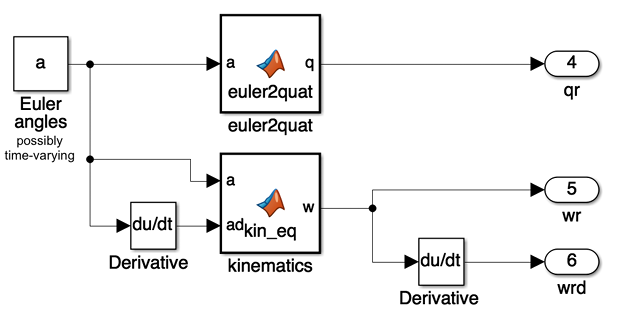
\includegraphics[scale=0.8]{AerospaceApplications/images/ref_gen.png}
    \caption{Simulink scheme for a reference generator}
\end{figure}


